\documentclass[conference]{IEEEtran}
\IEEEoverridecommandlockouts
% The preceding line is only needed to identify funding in the first footnote. If that is unneeded, please comment it out.
\usepackage{cite}
\usepackage{amsmath,amssymb,amsfonts}
\usepackage{algorithmic}
\usepackage{graphicx}
\usepackage{textcomp}
\usepackage{xcolor}
\usepackage[a4paper, total={184mm,239mm}]{geometry}
\def\BibTeX{{\rm B\kern-.05em{\sc i\kern-.025em b}\kern-.08em
    T\kern-.1667em\lower.7ex\hbox{E}\kern-.125emX}}
\usepackage{cleveref}
\usepackage{flexisym}
\usepackage{enumitem}
\usepackage{color}
\usepackage{graphicx}
\usepackage{booktabs}
\usepackage{listings}
\usepackage{xspace}
\usepackage{multicol}
\usepackage{float}
\usepackage{booktabs}
\usepackage{array}
\usepackage{url}
\lstset{
  backgroundcolor=\color{backcolour},   
  commentstyle=\color{codegreen},
  keywordstyle=\color{magenta},
  language = Prolog,
  literate = {-}{-}1,
  breaklines=true, 
  numbers=left,
  basicstyle=\sffamily,
  %keywordstyle=\bfseries,
  %morekeywords={reached,  in, source, sink,edge,node},
}
\usepackage{xcolor}
\definecolor{codegreen}{rgb}{0,0.6,0}
\definecolor{codegray}{rgb}{0.5,0.5,0.5}
\definecolor{codepurple}{rgb}{0.58,0,0.82}
\definecolor{backcolour}{rgb}{0.95,0.95,0.92}
\newtheorem{theorem}{Theorem}
\newtheorem{proposition}{Proposition}
\newtheorem{lemma}{Lemma}
\newtheorem{example}{Example}
\newtheorem{definition}{Definition}
\newtheorem{remark}{Remark}
\newtheorem{proof}{Proof}

\newcommand{\unsat}{\ensuremath{\mathsf{unsat}}}
\newcommand{\pos}[1]{\ensuremath{\mathsf{pos}(#1)}}
\newcommand{\ngt}[1]{\ensuremath{\mathsf{neg}(#1)}}
\newcommand{\cls}[1]{\ensuremath{\mathsf{c}(#1)}}
\newcommand{\vrbl}[1]{\ensuremath{\mathsf{v}(#1)}}
\newcommand{\program}[1]{\mathcal{P}(#1)}
\newcommand{\body}[1]{\mathsf{Body}(#1)}
\newcommand{\true}{\ensuremath{\mathsf{true}}\xspace}
\newcommand{\false}{\ensuremath{\mathsf{false}}\xspace}
\newcommand{\copyatom}[1]{#1\textprime}
\newcommand{\mmodel}[1]{\mathsf{MM}(#1)}
\newcommand{\Card}[1]{|#1|}
\newcommand{\Var}[1]{\mathsf{Var}(#1)}
\newcommand{\clarknot}{\ensuremath{\mathsf{not}}\text{ }}
\newcommand{\answer}[1]{\mathsf{AS}(#1)}
\newcommand{\toolname}{\ensuremath{\mathsf{MUS}}-\ensuremath{\mathsf{ASP}}}
\newcommand{\marco}{MARCO}
\newcommand{\unimus}{UNIMUS}
\newcommand{\remus}{ReMUS}
\newcommand{\be}{\mathbb{B}}
\begin{document}

\title{Computing MUS by ASP Solving}

\author{\IEEEauthorblockN{Mohimenul Kabir}
\IEEEauthorblockA{\textit{School of Computing} \\
\textit{National University of Singapore}\\
Singapore}
\and
\IEEEauthorblockN{Kuldeep S Meel}
\IEEEauthorblockA{\textit{Dept. of Computer Science} \\
\textit{University of Toronto}\\
Canada}
}

\maketitle

\begin{abstract}

\end{abstract}

\begin{IEEEkeywords}
component, formatting, style, styling, insert
\end{IEEEkeywords}

\section{Methodology}
In this section, for a given Boolean formula $F$, we introduce an ASP program where each answer set of the program correspondences to the unsatisfiable cores of $F$.
Finally, we introduce some optimization techniques to improve computational efficiency.  
\subsection{ASP Encoding}
For a given Boolean formula $F$, we introduce an ASP program $\program{F}$.
The ASP program $\program{F}$ involves introducing some ASP atoms as follows:
\begin{itemize}
  \item $\cls{i}$: for each clause $C_i \in F$, we introduce a free or choice atom $\cls{i}$
  
  The choice atom $\cls{i}$ indicates that the corresponding clause $C_i$ is under consideration. 
  \item $\pos{x}$, $\ngt{x}$: for each variable $x \in \Var{F}$. 
  
  We adapt the following symbolic interpretations: $\pos{x}$ ($\ngt{x}$ resp.) interprets that variable $x$ is assigned to \true (\false resp.). While 
  a variable cannot be assigned both values simultaneously, in our program $\program{F}$, it is likely that some its interpretations contains both $\pos{x}$ and $\neg{x}$ simultaneously. 
  \item $\unsat$: we introduce an atom $\unsat$ to denote that at least one of the under consideration clauses is unsatisfied.
\end{itemize}
\begin{lstlisting}[caption={Program $\program{F}$},label={code:as_to_uc},captionpos=b,mathescape=true,escapechar=|,float]
  % for each variable $x \in X$
  $\pos{x} \vee \ngt{x}$.|\label{line:each_variable}|
  % for each clause $C_i = x_1 \vee \ldots x_{k}, \vee \neg{x_{k+1}} \vee \ldots \neg{x_{k+m}}$
  $\unsat \leftarrow \cls{i}, \ngt{x_1}, \ldots \ngt{x_k}, \pos{x_{k+1}}, \ldots \pos{x_{k+m}}$.|\label{line:reach1}|
  % at least one clause must be falsified
  $\leftarrow$ not $\unsat$.|\label{line:unsat}|
  % for each variable X
  $\pos{x} \leftarrow \unsat$.
  $\ngt{x} \leftarrow \unsat$.
  % for each clause $C_i$, there is one free variable
  $\{ \cls{1}\text{ }; \ldots \text{ }\cls{n} \}.$|\label{line:all_clauses}|
\end{lstlisting}
\begin{lstlisting}[caption={Reduct of $\program{F}$ w.r.t. $M$},label={code:program_to_reduct},captionpos=b,mathescape=true,escapechar=|,float]
  % for each variable $x \in X$
  $\pos{x} \vee \ngt{x}$|\label{line:each_variable}|
  % for each clause $C_i \in M$
  $\unsat \vee \neg \cls{i} \vee \neg \ngt{x_1} \vee \ldots \vee \neg \ngt{x_k} \vee \neg \pos{x_{k+1}} \vee \ldots \vee \neg \pos{x_{k+m}}$|\label{line:reach1}|
  % for each variable X
  $\pos{x} \vee \neg \unsat$
  $\ngt{x} \vee \neg \unsat$
  % for each clause $c_i \in M$
  $\cls{i}$
\end{lstlisting}

Among the atoms of $\program{F}$, the atom $\cls{i}$ correspondences to clause $C_i \in F$. 
An interpretation $M$ over the atoms of $\program{F}$ considers a set of clauses of $F$.
More specifically, if $\cls{i} \in M$ then clause $C_i$ is considered by interpretation $M$.
We use the notation $M_{\downarrow \cls{.}}$ to denote the considered clauses under an interpretation. 
With the above set of atoms, given a Boolean formula $F = \bigwedge_{i=1}^{n} C_i$, we introduce an ASP program $\program{F}$ such that each of the unsatisfiable cores of $F$ one-to-one corresponds to answer sets of $\program{F}$. 
The ASP program $\program{F}$ is introduced in Listings~\ref{code:as_to_uc}. 
Moreover, we analyze the reduct of $\program{F}$, which is important for the theoretical analysis of the encoding. The theoretical guarantee of the program is established in~\Cref{lemma:as_to_uc_proof}.
\begin{lemma}
  \label{lemma:as_to_uc_proof}
  Each answer set $\sigma \in \answer{\program{F}}$ one-to-one corresponds to an unsatisfiable core of $F$.
\end{lemma}
\begin{proof}
  The lemma has two parts to proof:
  \begin{enumerate}
    \item For each $\sigma \in \answer{\program{F}}$, $\sigma_{\downarrow \cls{.}}$ corresponds to an unsatisfiable core of $F$
    \item Each unsatisfiable core $U$ of $F$ corresponds to an answer set of $\program{F}$ 
  \end{enumerate}
  Proof of `Part $1$': For an answer set $\sigma \in \answer{\program{F}}$, let assume $\sigma_{\downarrow c/1} = \{c_{i_1}, \ldots, c_{i_k}\}$.
  We proof that the clause set of $\sigma_{\downarrow c/1}$ constitutes an unsatisfiable core of $F$.

  Under answer set semantics, $\unsat \in \sigma$ (line~\ref{line:unsat} of encoding~\ref{code:as_to_uc}) and $\forall x \in \Var{F}$, $\{\pos{x}, \ngt{x}\} \subset \sigma$.
  Under clark completion semantics, since $\unsat \in \sigma$, $\exists r \in \program{F}$ such that 
  $\body{r}$ is evaluated to $\true$, which follows that there is a clause $C_i$ such that 
  $\cls{i} \in \sigma$ and for each $x \in c_i$, $\ngt{x} \in \sigma$ and $\neg{x} \in c_i$, $\pos{x} \in \sigma$.
  Note that $\forall x \in \Var{F}$, $\{\pos{x}, \ngt{x}\} \subset \sigma$, which interprets that each variable is assigned to both \true and \false.
  It follows that within the set of clause $\sigma_{\downarrow c/1}$, the clause $c_i$ is not satisfied even after assigning each variable to both \true and \false. 
  Thus, the clause set $\sigma_{\downarrow \cls{.}}$ constitutes a unsatisfiable core of $F$.

  Proof of `Part $2$': Let assume that the clause set $U = \{c_1, \ldots c_n\}$ is a unsatisfiable core of $F$.
  We proof that the clause set $U$ corresponds to an answer set of $\program{F}$. We show that given $U = \{c_{i_1}, \ldots c_{i_n}\}$, 
  $\sigma = \{\cls{i_1}, \ldots, \cls{i_n}\} \cup \{\unsat\} \cup \{\pos{x}, \ngt{x}| \forall x \in \Var{F}\}$ is an answer set of $\program{F}$.
  
  It is trivial to show that $\sigma \models \program{F}$. We show that  $\sigma$ is a minimal model of $\program{F}^{\sigma}$ by showing that each atom of $\sigma$ is justified in $\program{F}^{\sigma}$. 
  The $\program{F}^{\sigma}$ is a propositional encoding~\ref{code:program_to_reduct}.
  Since $\unsat \in \sigma$, there is no clause corresponding to the rule in line~\ref{line:unsat}. 
  Note that since $U$ is an unsatisfiable core of $F$, there exists a clause $C_{i_k} \in U$, $k \in [1,n]$ such that $C_{i_k}$ is not satisfied.
  Following the particular clause of $\program{F}^{\sigma}$, which contains the literal $\neg \cls{i_k}$, the atom $\unsat$ is justified. 
  Moreover, $\unsat \in \sigma$ implies that $\forall x \in \Var{F}$, both $\pos{x}$ and $\ngt{x}$ are also justified.
  Since each atom within $\sigma$ is justified, $\sigma$ is a minimal model of $\program{F}^{\sigma}$. It completes the proof. 
\end{proof}
The encoding~\ref{code:as_to_uc} computes all unsatisfiable cores of $F$ via a reduction to answer set solving. Thus, all subset minimal answer sets 
with respect to $\cls{.}$ corresponds to minimal unsatisfiable subsets of $F$.
\begin{proposition}
The subset minimal answer set of $\program{F}$ w.r.t. $\cls{.}$ correspondences to MUS of $F$.
\end{proposition}

\subsection{Optimizations to MUS Computation}
With Encoding~\ref{code:as_to_uc}, we add some additional constraints to speed up the MUS computation. 
The optimization techniques stem from the observations exploited in counting MUSes~\cite{BM2021}.
In this paper, we use some of their observations in computing MUSes. 

\paragraph{Minimum and Maximum Size of MUSes.}
If we can compute a minimum (or a lower bound) and maximum (or an upper bound) size of MUSes, then we can encode the cardinality information as an ASP cardinality constraints to reduce the search space of answer sets. 
We employ the same techniques exploited in~\cite{BM2021} to compute a lower and upper bound on the sizes of MUSes and modify the choice rule (Line~\ref{line:all_clauses} of Encoding~\ref{code:as_to_uc}) to a cardinality rule. 

\paragraph{Component Decompositions.}
Bendik and Meel~\cite{BM2021} partitions the clauses into {\em disjoint components} such that each clause of a MUS comes from the same component. 
The computation of disjoint components involves constructing a graph, similar to {\em flip graph}, which is often used in MUS extraction~\cite{Wieringa2012}.
To reduce the search space using the idea of disjoint components, our encoding adds a constraint as: $\leftarrow \cls{i}, \cls{j}$, for any two clauses $C_i$ and $C_j$ from two different components.   

\paragraph{Hitting Set Duality.}
Each of MUS of $F$ is a {\em minimal hitting set} of all of its MCSes~\cite{DW1987,Reiter1987}.
Thus, each MUS of $F$ contains some clauses from each MCS. 
This observation is also exploited by~\cite{BM2021} and similar to that, we compute the MCS of a formula with some time limit. 
To exploit the hitting set duality, we add a constraint as $\leftarrow \clarknot \cls{i_1}, \ldots, \clarknot \cls{i_k}$, 
where the clause set $C_{i_1}, \ldots, C_{i_k}$ constitutes an MCS of $F$.
\section{Experimental Evaluation}
\label{section:experiment}
To evaluate our prototype~\toolname, we conducted a detailed experimental evaluation on the available MUS benchmarks.
The objective of the experimental evaluation is to evaluate the performance of \toolname~with the existing MUS enumerators.

\subsection{Benchmark and Baseline}
We collected our benchmark from two areas:~(i)~MUS track of the SAT $2011$ competition~(ii)~scalable benchmark\footnote{\url{https://gitlab.com/satisfiability/scalablesat}} 
from MUS counting~\cite{BM2020}. We compare our prototype with three MUS enumeration tools: 
~(i)~\marco~\cite{LPMM2016}~(ii)~\unimus~\cite{BC2020}~and~(iii)~\remus~\cite{BCB2018}.

\subsection{Environmental Settings}
All experiments were conducted on a high-performance computing cluster equipped with nodes featuring AMD EPYC $7713$ CPUs, each with $128$ real cores. 
%We imposed a runtime limit of 5000 seconds and a memory cap of 16GB for each experiment.
%All experiments were carried out on a high-performance computer cluster, where each node consists of AMD EPYC $7713$ CPUs running with $128$ real cores. 
Throughout the experiment, the runtime and memory limits were set to $3600$ seconds and $16$GB, respectively, for all considered tools.

\subsection{Experimental Result}
We present the performance of all MUS enumerators in~\Cref{table:mus_enumeration_result}.
To compare the performance, the table shows the number of solveds instances of all MUS enumerators and their corresponding PAR-$2$ scores.
An instance is considered to be solved by a tool if the tool is able to enumerate all of its MUSes. 
The table clearly demonstrates that \toolname~outperforms existing MUS enumerators.
\begin{table}[h]
    \centering
    \begin{tabular}{m{5em} m{3em} m{3em} m{3em} m{5em}} 
    \toprule
    % & & \rotatebox{60}{\clingo} & \rotatebox{60}{DynASP} & \rotatebox{60}{Ganak}  & \rotatebox{60}{ApproxMC} & \rotatebox{60}{ApproxASP} \\ 
     & \marco & \unimus & \remus & \toolname\\
    \midrule
    \#Solved ($983$) & 248 & 248 & 245 & 547\\
    \midrule
    PAR-$2$ & 5422 & 5417 & 5441 & 3226\\
    \bottomrule
    \end{tabular}
    \caption{The performance of \toolname~vis-a-vis different MUS solvers.}
    \label{table:mus_enumeration_result}
\end{table}
\begin{figure}
    \centering
    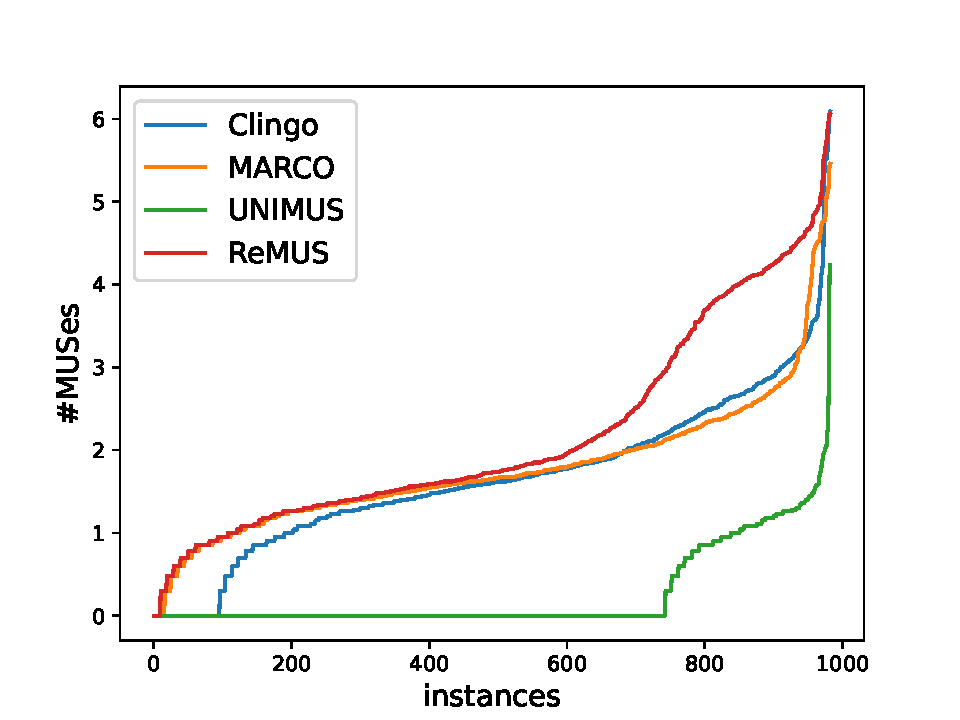
\includegraphics[scale=0.5]{images/countMUS.pdf}
    \caption{The number of MUSes enumerated by \toolname~by vis-a-vis other enumerators.}
    \label{fig:number_of_mus}
\end{figure}



% \begin{thebibliography}{00}
% \bibitem{b1} G. Eason, B. Noble, and I. N. Sneddon, ``On certain integrals of Lipschitz-Hankel type involving products of Bessel functions,'' Phil. Trans. Roy. Soc. London, vol. A247, pp. 529--551, April 1955.
% \bibitem{b2} J. Clerk Maxwell, A Treatise on Electricity and Magnetism, 3rd ed., vol. 2. Oxford: Clarendon, 1892, pp.68--73.
% \bibitem{b3} I. S. Jacobs and C. P. Bean, ``Fine particles, thin films and exchange anisotropy,'' in Magnetism, vol. III, G. T. Rado and H. Suhl, Eds. New York: Academic, 1963, pp. 271--350.
% \bibitem{b4} K. Elissa, ``Title of paper if known,'' unpublished.
% \bibitem{b5} R. Nicole, ``Title of paper with only first word capitalized,'' J. Name Stand. Abbrev., in press.
% \bibitem{b6} Y. Yorozu, M. Hirano, K. Oka, and Y. Tagawa, ``Electron spectroscopy studies on magneto-optical media and plastic substrate interface,'' IEEE Transl. J. Magn. Japan, vol. 2, pp. 740--741, August 1987 [Digests 9th Annual Conf. Magnetics Japan, p. 301, 1982].
% \bibitem{b7} M. Young, The Technical Writer's Handbook. Mill Valley, CA: University Science, 1989.
% \end{thebibliography}
\bibliographystyle{IEEEtran}
\bibliography{template-A4}
\vspace{12pt}
\color{red}
\end{document}
